\documentclass{article}
\usepackage{amsmath}
\usepackage{xcolor}
\usepackage{amsthm}
\usepackage{graphicx}
\usepackage{hyperref}
\usepackage{datetime}
\usepackage{todonotes}

\graphicspath{ {../} }

\usepackage[margin=3.5cm,a4paper]{geometry}

% inline comments
% you could use \listoftodos to print an overview
\newcommand{\inline}[1]{ {\color{blue}{#1}}\addcontentsline{tdo}{todo}{#1}}
\newcommand{\comment}[1]{{\color{blue}\noindent{#1}\\}\addcontentsline{tdo}{todo}{#1}}
% use this one to disable
%\newcommand{\inline}[1]{\ignorespaces}


\newdateformat{monthyeardate}{\monthname[\THEMONTH] \THEYEAR}

\newcommand{\newmarkedtheorem}[1]{%
  \newenvironment{#1}
    {\pushQED{\qed}\csname inner@#1\endcsname}
    {\popQED\csname endinner@#1\endcsname}%
  \newtheorem{inner@#1}%
}

\theoremstyle{definition}
%\newtheorem{eg}{Example}[section]
\newmarkedtheorem{eg}{Example}[section]
\newtheorem{observation}{Observation}[section]
\theoremstyle{plain}
\newtheorem{define}{Definition}[section]
\newtheorem{proposition}{Proposition}[section]
\newtheorem{theorem}{Theorem}[section]
\newtheorem{assump}{Assumption}[section]
\newtheorem{remark}{Remark}[section]


\title{Traffic Scheduling - Project Outline}
\author{Jeroen van Riel}
\date{\monthyeardate\today}

\begin{document}

\maketitle

% problem exploration and definition
% - context
%   - autonomous vehicle
%   - possible applications
% - general trajectory finding problem
% - example of reduction to scheduling

% research plan
% - reading (theory and literature)
% - writing
% - modeling
% - experiments

% proposal
% - concrete contributions
%   - general problem formulation
% - using ML for combinatorics
% - traffic context
%   - personal interest
%   - applictions (warehouse navigation)

\section{Introduction}

Given the growing number of autonomous vehicles, an interesting question becomes
how efficient traffic can be handled in a situation where every individual
vehicle can be fully controlled by a single traffic manager with full
information and perfect communication. Studying this question is important,
because it gives us an idea of the best we can do in an idealized situation,
without considering issues such as decentralized control, communication latency
and partial information.


\section{Traffic Problem}

We will start by introducing a traffic scheduling problem that forms the basis
of the entire project.

Consider a very abstract problem in which vehicles
represented as little dots are moving over a graph in a continuous fashion.
Vehicles arrive to the graph over time and need to follow a fixed route towards
a final node, where the vehicle leaves the system. The goal of the traffic
controller is to determine how vehicles move exactly along their route, while
satisfying some constraints on the interaction between vehicles that are based
on safety considerations.

% introduce network graph
Let the traffic network be modeled as a weighted directed graph $G=(V,E)$, with
nodes and arcs representing intersections and roads, respectively. Vehicles can
travel along a series of arcs that are connected. Each node of degree one is
called an \textit{external node} and models the location where vehicles enter
(\textit{entrypoint}) or exit (\textit{exitpoint}) the network. A node of degree
at least three is called an \textit{intersection}.

% behavior (traveling through the network)
For each vehicle $j$, let its route be denoted by $R_{j}$, which is encoded as a
sequence of nodes. Vehicle $j$ enters the network at some external node
$R_{j}(0)$ at time $t^{0}_{j}$ and then visits the $n_{j}$ intersections
$R_{j}(1), \dots, R_{j}(n_{j})$ until it reaches the exitpoint
$R_{j}(n_{j} + 1)$, where it leaves the network.
% define common path
Given two routes $R_{j}$ and $R_{l}$, we define a \textit{common path}
$P=(i_{1},\dots,i_{L})$ as a substring of some length $L$ of both routes
(including external nodes). We refer to the first node $i_{1}$ of a common path
as a \textit{merge point}. The set of all common paths for vehicles $j$ and $l$
is denoted $P_{jl}$. See Figure~\ref{fig:intersection-graph-example} for an
illustration of the above concepts.

\begin{figure}[t]
  \centering
  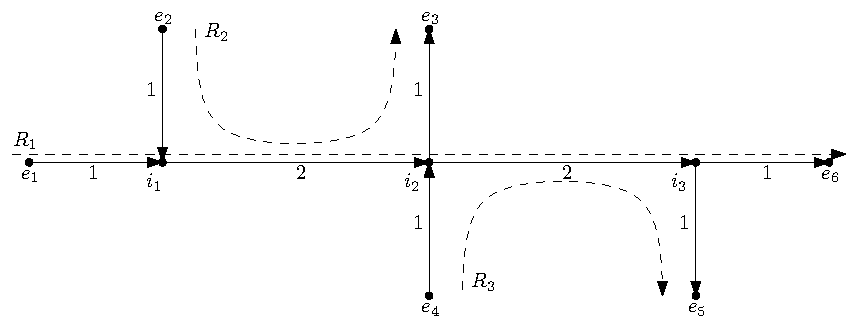
\includegraphics[width=1.0\textwidth]{figures/intersection-graph-example.pdf}
  \label{fig:intersection-graph-example}
  \caption{Example graph with three intersection $i_{1}, i_{2}, i_{3}$ and three
    vehicles, for which the routes are indicated by $R_{1}, R_{2}$ and $R_{3}$.
    The external nodes are labeled as $e_{1}, \dots, e_{6}$. The weight
    (travel time) of each arc is indicated next to it. The common paths are
    $P_{12} = \{ (i_{1}, i_{2}) \}$, $P_{13} = \{ (i_{2}, i_{3}) \}$
    $P_{23} = \{ (i_{2}) \}$ and the corresponding merge points are
    $M_{12} = \{ i_{1} \}, M_{13} = \{ i_{2} \}, M_{23} = \{ i_{2} \}$.}
\end{figure}

Let $x_{j}(t)$ denote the position of vehicle $j$ on its route $R_{j}$ at time
$t \geq t_{j}^{0}$. We also use the notation $x_{ij}(t)$ to denote the position
on the lane on the route of $j$ leading to the $i$th intersection on its route.
Furthermore, let $v_{j}(t)$ and $a_{j}(t)$ denote the speed and acceleration,
respectively, of vehicle $j$ at time $t$.

\begin{figure}[b]
  \centering
  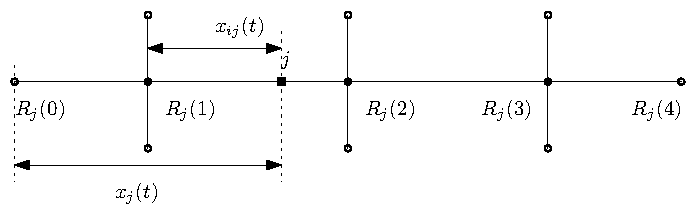
\includegraphics[width=0.9\textwidth]{figures/general_traffic_model.pdf}
  \caption{Illustration of a network of intersections with the position of some
    vehicle $j$ given in two ways.}
  \label{fig:general-model}
\end{figure}

% trajectory constraints: smoothness, velocity and acceleration
The task of the traffic controller is to determine trajectories $x_{j}$ (or
equivalently either $v_{j}$ or $a_{j}$) satisfying some kind of smoothness and
safety constraints. For example, we may impose maximum/minimum speed and
acceleration constraints
\begin{align}
    v_\text{min} & \leq v_j(t) \leq v_\text{max} , \\
    a_\text{min} & \leq a_j(t) \leq a_\text{max} .
\end{align}


% lane switching: merge point (head of common path)
Given a node $i$, we will use $t_{ij} = t_{ij}(x_{j})$ to denote the time when
vehicle $j$ crosses $i$. Between crossing of vehicles from different lanes, we
enforce a \textit{safe lane-switching} time $s_{\text{lane}}$. At each merge
point $i_{1}$ of each path $P = (i_{1}, \dots, i_{L}) \in P_{jl}$ for all pairs
of distinct vehicles $\{j,l\}$, we require that either
\begin{align}
  t_{ij} + s_{\text{lane}} \leq t_{il} \quad \text{ or } \quad t_{il} + s_{\text{lane}} \leq t_{ij} .
\end{align}
% following distance and overtaking: tail of common path
Furthermore, when two vehicles $j$ and $l$ are driving on the same lane we require some
minimum \textit{safe following distance} $d_{\text{follow}}$. For all pairs of
distinct vehicles $\{j,l\}$, for each common path
$P = (i_{1}, \dots, i_{L}) \in P_{jl}$, we require for each intersection
$i \in P \setminus \{ i_{1} \}$ that
\begin{align}
  \label{eq:following-distance-constraint}
  x_{ij}(t) + d_{\text{follow}} \leq x_{il}(t) \quad \text{ or } \quad x_{il}(t) + d_{\text{follow}} \leq x_{ij}(t) ,
\end{align}
for all $t$ in the time interval when both vehicles are driving on the common
path. When we do not allow vehicles to overtake each other, exactly one of the
inequalities must hold for the entire common path. For simplicity, this second
type of constraints was stated in terms of distance, but note that it could be
equivalently stated in terms of time as well.

\subsection{Optimization setting}

\begin{figure}
  \centering
  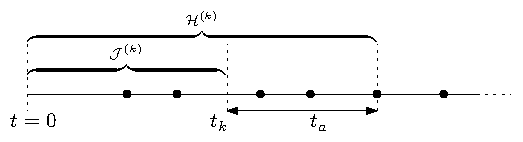
\includegraphics[width=1.0\textwidth]{figures/sequential-decision-process.pdf}
  \caption{Illustration of some decision epoch $t_{k}$ and the corresponding set
    of vehicles under control and the visible horizon. The dots represent vehicle
    arrival times $t_{j}^{0}$.}
  \label{fig:sequential-decision-process}
\end{figure}

Let us now consider more precisely how the controller interacts with the system
defined above.
In general, at some time $t$, we assume that the controller knows the arrival
times of vehicles
\begin{align}
  \mathcal{H}_{t} = \{ j : t_{j}^{0} \leq t + t_{\text{a}}\} ,
\end{align}
for some non-negative look-ahead time $t_{\text{a}}$. We call this set of
vehicles (with their corresponding arrival times) the \textit{visible horizon}
of the controller. Similarly, let the set of vehicles in the system at time $t$
be denoted by
\begin{align}
  \mathcal{J}_{t} = \{ j : t_{j}^{0} \leq t \} .
\end{align}
Ignoring for now that vehicles eventually leave the system, we say that
$\mathcal{J}_{t}$ are precisely the vehicles \textit{under control} of the
traffic controller.

Note that the only uncertainty in the system stems from the random arrival times
of vehicles. Once trajectories are determined, the dynamics of the system are
completely deterministic as long as $\mathcal{H}_{t}$ does not change.
Therefore, the only sensible decision epochs to consider are the points in time
$t_{k}$ whenever $\mathcal{H}_{t}$ changes, i.e., when new information becomes
available, see Figure~\ref{fig:sequential-decision-process} for an illustration.
Whenever this happens, the controller needs to compute a trajectory for the
newly arrived vehicles, and is free to revise the trajectories of the vehicles
that are already in the system. However, these updated trajectories need to
respect the trajectories that have been followed up till that point.

Let us make the sequential decision process sketched above a little bit more
precise. To simplify notation, we define
$\mathcal{J}^{(k)} = \mathcal{J}_{t_{k}}$ and
$\mathcal{H}^{(k)} = \mathcal{H}_{t_{k}}$. Let the \textit{state} of the system
at time $t_{k}$ be represented by the sets
\begin{align}
  s_{k} = (\{(t_{j}^{0}, R_{j})\}_{j \in \mathcal{H}^{(k)}}, \;
  \{(x_{j}^{(k-1)}(t_{k}), v_{j}^{(k-1)}(t_{k}), a_{j}^{(k-1)}(t_{k}))\}_{j \in \mathcal{J}^{(k)}} ) .
\end{align}
The controller needs to compute a set of trajectories
\begin{align}
a_{t} = \{ x_{j}^{(k)}\}_{j \in \mathcal{H}^{(k)}} ,
\end{align}
which are functions of $t \geq t_{j}^{0}$, satisfying the constraints from the
previous section and the additional constraints
\begin{subequations}
\begin{align}
  x_{j}^{(k)}(t_{k}) = x_{j}^{(k-1)}(t_{k}), \\
  v_{j}^{(k)}(t_{k}) = v_{j}^{(k-1)}(t_{k}), \\
  a_{j}^{(k)}(t_{k}) = a_{j}^{(k-1)}(t_{k}),
\end{align}
\end{subequations}
for the vehicles $j \in \mathcal{J}^{(k)}$ that were already under control,
guaranteeing in some sense the \textit{continuation} of the updated
trajectories.

From the above discussion, it should be clear that the transition to the next
state $s_{k+1}$ is particularly simple. The arrivals that happen at
$t_{k+1} + t_{a}$ are simply added to the visible horizon and the positions,
speeds and accelerations follow directly from the determined trajectories
$a_{t}$.

% TODO: vehicles leaving the network (could choose to let them stay at R_j(n_j))

% objective
We still have to define an objective to compare the performance of different
controllers. Measures of how well the controller performs on some particular
sequence of arriving vehicles may be based on properties of the computed
trajectories. For example, we could relate some measure of energy consumption to
acceleration, or we can measure delay based on the crossing times $t_{ij}$. In
general, the optimization objective is the expected value of this measure, where
the expectation is taken over the distribution of the vehicle arrival process.

% horizon
Finally, we may distinguish between a finite-horizon problem with a finite
number of vehicles, or an infinite-horizon case, in which particular attention
needs to be paid to the definition of the optimizaton objective, e.g., we might
need to use discounting to avoid infinite sums.


\section{Analysis}

Before discussing concrete models for solving the general traffic scheduling
problem, let us discuss two important aspects that will be relevant throughout
the analysis of all the models and the corresponding reinforcement learning
formulations.

% arrival distribution

First of all, we need to make some assumptions on how vehicles arrive to the
network. We assume that each vehicle $j$ has an earliest arrival time $r_j$. The
controller decides the exact arrival time $t^{0}_j \geq r_j$ when the vehicle
actually enters the network. By having this assumption, we make sure that the
problem is always feasible, because vehicles can be kept waiting at the
entrypoints for as long as necessary. Would we assumed that vehicle are forced
to enter the network at their arrival time $r_j$, it is not difficult to see
there are instances in which no trajectories satisfy the safety constraints.

% generalization

An interesting aspect of any learned policy is its generalization to similar
problems. It would be interesting to study generalization across different
network topologies, starting with trying to formulate a policy that is agnostic
to the network topology. More straightforward would be the study of
generalization across different arrival distributions. It is well known that
road traffic demand fluctuates highly throughout the day. Therefore, a policy
that keeps good performance under increased arrival rates is desirable. An
interesting next step would be to see if an explicit memory mechanism could
improve the ability to adapt to changing arrival rates.


\section{Research Plan}

In order to compute trajectories for the general traffic control problem
sketched above, we propose some models that are all based on some kind of
discretization. This allows us to formulate a policy space for which we can use
reinforcement learning techniques for finding good policies. The following
subsections will shortly introduce the three main kinds of models that we want
to consider, ordered by increasing complexity.


\subsection{Single Intersection}

% reduction to offline scheduling

A trajectory generating approach for a single intersection has been proposed in
\cite{timmermanPlatoonFormingAlgorithms2021}. The main idea is to first schedule the times at which vehicles
cross the intersection and then generate feasible trajectories accordingly. When
the objective only measures delay at the intersection, this shows that the
single intersection problem reduces to scheduling crossing times at the
intersection. More precisely, in machine scheduling terminology, we are dealing
with a single machine scheduling problem with release dates, job families with
chain precedence constraints (corresponding to lanes), family-dependent setup
times and total completion time objective. Furthermore, the platoon preservation
theorem from \cite{limpensOnlinePlatoonForming2023} lowers the complexity of the problem even further.
Under the assumption that all future arrivals are known, the problem can be
solved to optimality by formulating it as a Mixed-Integer Linear Program (MILP).
Nevertheless, it makes sense to study heuristic method that would allow us to
tackle larger instances.

% online scheduling

When we drop the assumption of complete knowledge of the future, we are in the
setting of online scheduling \cite{vestjensOnlineMachineScheduling1997}, in which vehicle arrival times
become gradually known to the controller over time. There are multiple ways to
assess the performance of an online scheduler, but the most straightforward way
is to study the competitive ratio compared with a so-called adversary. In case
of a deterministic algorithm, the adversary constructs a problem instance based
on the description of the algorithm and then solves it optimally. The worst-case
ratio between the objective value of the algorithm and the objective of the
optimal solution is called the competitive ratio. Following a similar approach
as in the proof of Theorem 2.1 in \cite{vestjensOnlineMachineScheduling1997}, we might be able to show a
lower bound on the competitive ratio. After some quick calculations, we found
that (for some particular problem parameters) this ratio is strictly larger than
1, which roughly means that there is some value in knowing the future. However,
the expressions that we obtained do not allow a clean analysis, so obtaining the
lower bound might require some numerical approximation.

% heuristics

Our goal is to study heuristics for the offline and online single intersection
scheduling problem. A common approach in the scheduling literature is to
manually formulate heuristics based on our understanding of the problem
structure. Instead, we will be using reinforcement learning techniques to
automatically learn heuristics. In order to apply reinforcement lenaring
techniques, we first need to precisely specify the interaction between the
controller and the environment, which is done by formulating a Markov Decision
Process. We will study an MDP that is based on the idea of \textit{dispatching},
which is an idea from scheduling theory in which a schedule is constructed by
iteratively choosing the next vehicle that is allowed to use a shared resource.
In this way, the learned policy is applicable in both the offline and online
problem setting.

% status and plan

We have a precise definition of the single intersection scheduling problem.
Furthermore, we formulated a MILP and have some code to solve arbitrary
instances exactly using the commerical Gurobi solver \cite{gurobi}. We have
implemented the dispatching MDP as a Gymnasium \cite{towers_gymnasium_2023}
environment and we have setup a basic DQN \cite{mnihHumanlevelControlDeep2015}
agent based on the off-the-shelf implementation of CleanRL
\cite{huang2022cleanrl}. What remains to be done is a thorough analysis of the
learned policies for different distributions of the vehicle arrival process.
Part of this analysis will be a comparison to the exact solutions found via the
MILP solver.


\subsection{Network}

% job shop

Next, we consider multiple intersections in a network. When we neglect the
dynamics of vehicles on lanes between intersections, a very natural formulation
of the scheduling problem is given by a job shop \cite{pinedoSchedulingTheoryAlgorithms2016} scheduling
problem with some additional constraints to encode the time that a vehicle needs
to travel to the next intersection on its route. In theory, it is still possible
to solve the offline variant exactly using a MILP solver. However, we expect
that this approach does not scale well in terms of the network size and number
of vehicles. Therefore, in order to solve real-world problems, we want to focus
on finding good heuristics.

% dispatching reinforcement learning

A natural extension of the dispatching approach that we used in the single
intersection case would be based on dispatching at every intersection. Like we
did for the single intersection case, this method could be compared to exact
solutions, but we expect that the scale of the problem will be prohibitive here.

% disjunctive graph

Some recent works
\cite{zhangLearningDispatchJob2020,tasselReinforcementLearningEnvironment2021}
have investigated reinforcement learning method for solving job shop problems
and showed some promising results. Therefore, we would like to investigate how
to use these methods to construct an efficient reinforcement learning
formulation for the offline variant. The method from
\cite{zhangLearningDispatchJob2020} uses the idea of a disjunctive graph
corresponding to the jobs shop problem. Determining the order of vehicles in the
schedule is equivalent to determining the directions of a certain set of arcs in
this disjunctive graph. A reinforcement learning controller can be learned to
iteratively direct these arcs based on an graph neural network embedding of the
current disjunctive graph.

% network effects

The model from \cite{timmermanPlatoonFormingAlgorithms2021} together with the
platoon preservation theorem \cite{limpensOnlinePlatoonForming2023} imply that
it is never beneficial to split platoons when there is only a single
intersection. However, for more than one intersections, we have found examples
where platoon splitting is necessary in the optimal schedule. It would be
interesting to understand better why this happens and characterize somehow these
kind of situations.


\subsection{Finite buffers}

% location delays

In the models discussed above, we assumed that vehicles do not interact on
lanes, hence it is possible for an unbounded number of vehicles to wait on a
lane at any given time. However, in real-world traffic networks, the allowed
number of vehicles is limited by space constraints and even depends non-trivally
on the speeds of individual vehicles. Therefore, we propose a model that
incorporates this aspect by considering the position of vehicles on lanes.
Instead of encoding the precise location in a continuous sense, we divide each
lane in a finite number of locations. For a given vehicle, the controller has to
decide how long it should wait on each location. For large number of locations
per lane, this method allows us to approximate continuous trajectories.

% more precise

In order to illustrate this kind of model, we will make the case with one
intersection a little bit more formal. Assume that it takes constant time
$\Delta t$ for a vehicle to travel to the next location. For each lane $k$, let
$m_{k}$ denote the number of locations, excluding the entrypoint. Let the
locations of lane $k$ be identified by increasing numbers
$\mathcal{L}(k) = (1, \dots , m_{k})$, where the last one corresponds to the
final intersection. In the following variable definitions, we will not
explicitly mention the dependency on the lane to keep notation simple. Let
$y_{ij}$ denote the time at which vehicle $j$ departs from location
$i \in \{ 0, \dots, m_{k} \}$, then $y_{ij} + \Delta t$ is the arrival time of
vehicle $j$ at location $i+1$. To simplify notation, we define
$\bar{y}_{ij} = y_{i-1,j} + \Delta t$ to be the arrival time of vehicle $j$ at
location $i$. For every location $i$ and vehicle $j$, we require
\begin{align}
  \label{eq:constr1}
  \bar{y}_{ij} \leq y_{ij} .
\end{align}
For each pair of consecutive vehicles on the same lane $k$ with precedence
constraint $j \rightarrow l \in \mathcal{C}_{k}$, we have the inequalities
\begin{align}
  \label{eq:constr2}
  y_{ij} + p \leq \bar{y}_{il} ,
\end{align}
for every location $i$ along their route. Furthermore, we assume that for every
vehicle $j$, the initial departure time from the entrypoint of vehicle $j$ satisfies
\begin{align}
  \label{eq:release}
 t^{0}_{j} \leq y_{0j}
\end{align}
in order to model the \textit{arrival time} of the vehicle.

Finally, we need to model the safety constraints involving vehicles from
different lanes that cross the intersection. Let $j$ be some vehicle on lane
$k(j)$, then let let $y_{j}$ denote the departure time from the intersection, so
we have $y_{j} = y_{ij}$ with $i=m_{k(j)}$. Similarly, let $\bar{y}_{j}$ denote
the arrival time of $j$ at the intersection, so we have
$\bar{y}_{j} = y_{i-1,j} + \Delta t$ with $i = m_{k(j)}$. From
constraints~\eqref{eq:constr2}, we see that it makes sense to say that vehicle
$j$ occupies the intersection during the interval
\begin{align}
  [\bar{y}_{j}, y_{j} + p] .
\end{align}
We require an additional \textit{switch-over time} $s$ whenever the next vehicle
to occupy the intersection comes from a different lane. Let
\begin{align}
  \mathcal{D} = \{ \{j, l\} : j \in F_{k_{1}}, l \in F_{k_{2}} , k_{1} \neq k_{2} \} ,
\end{align}
denote the set of \textit{conflict} pairs. The additional constraints are
\begin{align}
  \label{eq:3}
  y_{j} + p + s \leq \bar{y}_{l} \quad \text{ or } \quad y_{l} + p + s \leq \bar{y}_{j} ,
\end{align}
for all $j, l \in \mathcal{D}$.


% single intersection

When the objective only measures delay at the intersection, the case of a single
intersection reduces to the single intersection scheduling problem with infinite
lane capacity, because the entrypoints still have infinite capacity. Therefore,
a vehicle can wait as long as necessary at the entrypoint, before entering the
lane.

% network

Once we consider more than one intersection, the controller needs to start
taking into account the effects of finite lane capacity. Because of the discrete
nature of the model, it is straightforward to formulate it as a MILP, which
allows us to solve the problem exactly. However, as the number of variables
grows rapidly with the values of $m_{k}$, we do not expect this approach to
scale well.

% status and plan

We have started with proving that the single intersection case reduces to the
problem with infinite lane capacity. Furthermore, we have a MILP formulation
that we can solve with Gurobi, which we could use to verify this
reduction claim. We still need to make precise in what way our model
approximates the generation of continuous trajectories. Based on a suitable
definition, we should then prove that a certain error measure can be made
arbitrily small by choosing values for $m_{k}$ large enough.

Once we are done with the theoretical investigation sketched above, we should be
ready to start experimenting with reinforcement learning controllers. A major
question is how to structure the policy for determining location delays for
vehicles in a online setting. It might seem straightforward to have the
controller determine the location delays for a fixed number of upstream
locations, but it is not immediately clear how to define this for a variable
number of vehicles. One approach would be to have the controller set a location
delay for each location. Each time a vehicle enters a location, it will stay
there for the set location delay. This way, we have shifted the focus to the
infrastructure, similarly like we did in the dispatching environment for the
single intersection scheduling problem.


\bibliography{references}
\bibliographystyle{ieeetr}

\end{document}

